
\section{Results}

We generate the visibility graphs for each subregion of interest using the time-magnitude sequences \myrevision{of both the complete and declustered catalogs. In the case of the complete catalog, that corresponds to the sequences shown in Fig.~\ref{fig:mag-time}. In every case, the numbers of nodes in each graph are the same as those shown in Table \ref{tab:seismicity}; and} the links between inter-visible events are established following the condition in equation (\ref{eq:vg}), as in the example shown in Fig.~\ref{fig:vg}. (We do not include a visualization of the graphs because the links are so many, that it is only practical to visualize the graphs of short sequences.) We collect information about the number of inter-visibility links associated with each event (connectivity degree, $k$) and categorize the events in magnitude bins of size $\Delta M_{\mathrm{bin}} = 0.1$, as mentioned in the Methodology section. Figure \ref{fig:km} shows the scattered distribution of events in the magnitude-connectivity degree plane for each subregion\myrevision{, corresponding to the complete catalogs.} The figure shows that, in general, the value of $k$ increases with $M_w$\myrevision{; and includes the results of obtaining linear $k$-$M$ regressions for each dataset along with the values of the slope $m$ for the three seismic zones, namely 10.0, 9.85, and 8.70 for the Azerbaijan, Alborz, and Kopeh Dagh regions. Similar results regressions were obtained for the declustered catalogs, which yielded $m$ values of 8.92, 8.97, and 7.96, respectively.}

\begin{figure*}[t]
	\centering
	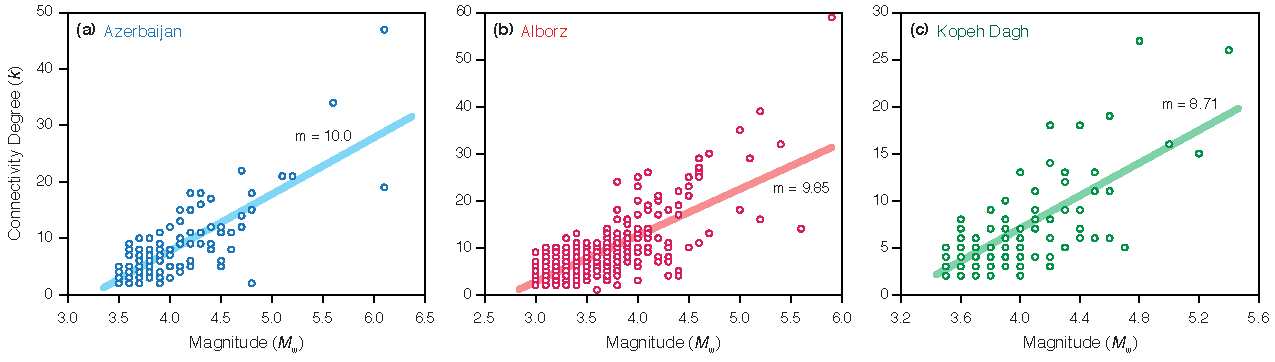
\includegraphics[width=\textwidth]{figures/pdf/figure-06} 
	\caption{Scattered distribution of events in the magnitude-connectivity degree plane and linear regressions obtained for the $k$-$M$ relationships for the three seismic regions in northern Iran. The value next to each of regression line corresponds to the slope of the line, which is referred here as the $k$-$M$ slope.}
	\label{fig:km}
\end{figure*}

Next, we examine the relationship between the $b$ values from Table \ref{tab:seismicity} and the $k$-$M$ slopes. \myrevision{Figures \ref{fig:regression}a and \ref{fig:regression}a show the scattered results of the $m$ versus $b$ for the complete and declustered catalogs, respectively. Along with the data-points obtained for our analysis of the three seismic regions of northern Iran, in each plot, we also include the data points corresponding to the magnitude-time sequences of the Mexican subduction zone provided by \citet{Telesca2013}, the Pannoninan seismic zone from \citet{Telesca2014}, the experimental results obtained by \citet{Telesca2014-pone}, and the result from a similar preliminary analysis done by \citet{Azizzadeh_2017_SSA} for California. These figures also include the linear trends of the data points, as they are aggregated (i.e., each regression reflects the addition of new data-points from different studies). In the figure, we indicate which data points were considered for each of the computed linear regressions and their corresponding correlation coefficient, $R$.}

\myrevision{Here, as well as in other figures, we present our results for both the complete and declustered catalogs to shed light upon the local differences for the case of northern Iran, and to contribute, globally, to the discussion of the appropriate treatment and selection of catalogs for the use of the visibility graph method. We note, for instance, that the data points in Fig.~\ref{fig:regression} from \citet{Telesca2012} and \citet{Telesca2013} used whole catalogs, whereas those from \citet{Telesca2014} and \citet{Telesca2016} used declustered catalogs.}

\myrevision{Note that, overall, the linear trends shown in Fig.~\ref{fig:regression} hold independently of the differences in the studies in terms of number of events, seismic characteristics, and the treatment of the catalogs. Also note that these trends tend to improve with increasing number of data points, as reflected by the increasing value of $R$. Regarding this, we should note that the data points in Fig.~\ref{fig:regression} cover what would otherwise be considered a large span of $b$ values. While we recognize that most earthquake data lead to $b$ values ranging between 0.8 and 1.2, it is also known that there are regions with low- and high-$b$ values \citep[e.g.,][]{Singh_1983_BSSA, Pacheco_1992_N, Nakaya_2006_JGR}. In addition, \citet{Scholz_1968_BSSA} reported that experimental microfractures in rocks, similar to those observed in earthquakes, exhibit $b$ values ranging between 0.11 and 2.58. Considering that, by definition, $b$ represents the proportion between the amount of large and small events in a region, the trends shown in Fig.~\ref{fig:regression} contribute to the suggestion made by \citet{Telesca2014} about the universal character of the relationship between $b$ and $m$.}

According to these results, a universal relationship between $b$ and $m$ can be expressed as
% 
\begin{equation}
\myrevision{
	b = 0.073 + 0.084 m
	\label{eq:universal.bm}
}
\end{equation}
%
\myrevision{for the case in which we consider the complete catalogs for northern Iran, and}
% 
\begin{equation}
\myrevision{
	b = 0.077 + 0.085 m
	\label{eq:universal.bm.dc}
}
\end{equation}
%
\myrevision{for the case in which we consider the declustered catalogs for northern Iran. This indicates that once combined with the data points of other regions, the option of considering either catalog leads to very similar results as, on average, the data points oscillate about the same universal relationship. Locally, however, for the case of northern Iran trends alone, it seems that the declustered catalog leads to a closer fit with the universal relationship. Separately (not shown here for brevity), we also observed that, for the particular sequences under study, the results seem to be more sensitive to less conservative values of $M_c$, as the choice of a smaller $M_c$ leads to larger datasets. \citet{Telesca2012} and \citet{Telesca2013}, however, pointed out that for sufficiently long sequences, the threshold magnitude have only small effects on the graph parameters.}

\begin{figure*}[t]
	\centering
	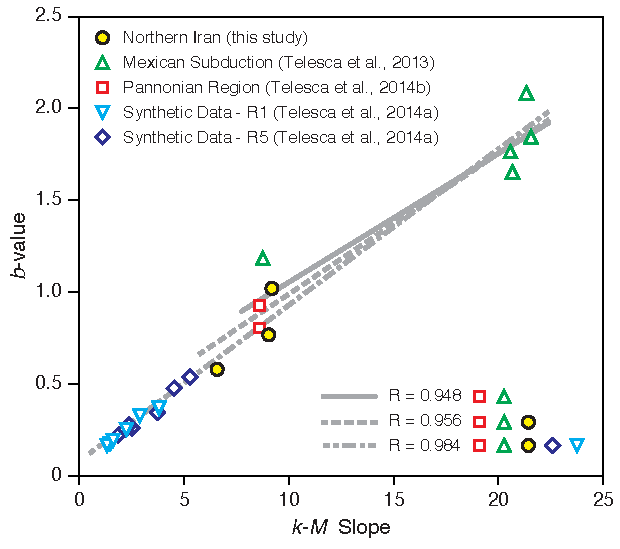
\includegraphics[width=\textwidth]{figures/pdf/figure-07} 
	\caption{\myrevision{Correlation between $k$-$M$ slope ($m$) and the $b$ value as drawn from the results of the present study for the region of northern Iranian using the complete (a) and declustered (b) catalogs, along with other previous studies including analysis of the Mexican subduction zone \citep{Telesca2013}, the Pannonian seismic zone \citep{Telesca2014}, southern California \citep{Azizzadeh_2017_SSA}, and results from two experiments \citep{Telesca2014-pone}. The lines represent linear regressions obtained to fit the different data points, considering different combinations. The values of the correlation coefficient, $R$, are indicated for each regression line.}}
	\label{fig:regression}
\end{figure*}

To further explore the sensitivity of the graph properties to the number of events in each catalog and the value of the minimum magnitude, we randomly picked a significant number of subsequences from within the initial catalog compiled for each region, and repeated the analysis for each subsequence. In total, for each region, we extracted 200 new subsequences from the \myrevision{whole} catalog. The number of events in each subsequence, $n$, was varied randomly but chosen to be large enough to represent the seismic characteristics of each region. In particular, the minimum size of each subsequence was set to be $n \geq 200$, and the maximum size in the sequence was set to be as large as the original \myrevision{whole} catalog (see Table \ref{tab:seismicity}). We forced the random subsequences to progress positively in time without altering the natural occurrence of events. In other words, we randomly determined the initial event and the subsequence size (number of events to be considered), and then picked that number of events following the initial earthquake in the subsequence. Next, we determined the value of $M_c$ and $b$ \myrevision{to obtain the complete and declustered catalogs for each region}, created the graph for all events with $M \geq M_c$, and extracted the connectivity degree of the events in each subsequence. \myrevision{Because this needed to be done for a large number of subsequences, in this part of the analysis we used the goodness-of-fit test (GFT) method to determine $M_c$ systematically, instead of the MAXC method. The GFT method follows the recommendations of \citet{Wiemer2000} and \citet{Wiemer2001}, and leads to less conservative values of $M_c$, which is preferable to keep the subsequences large enough.}

\begin{figure*}%[t]
	\centering
	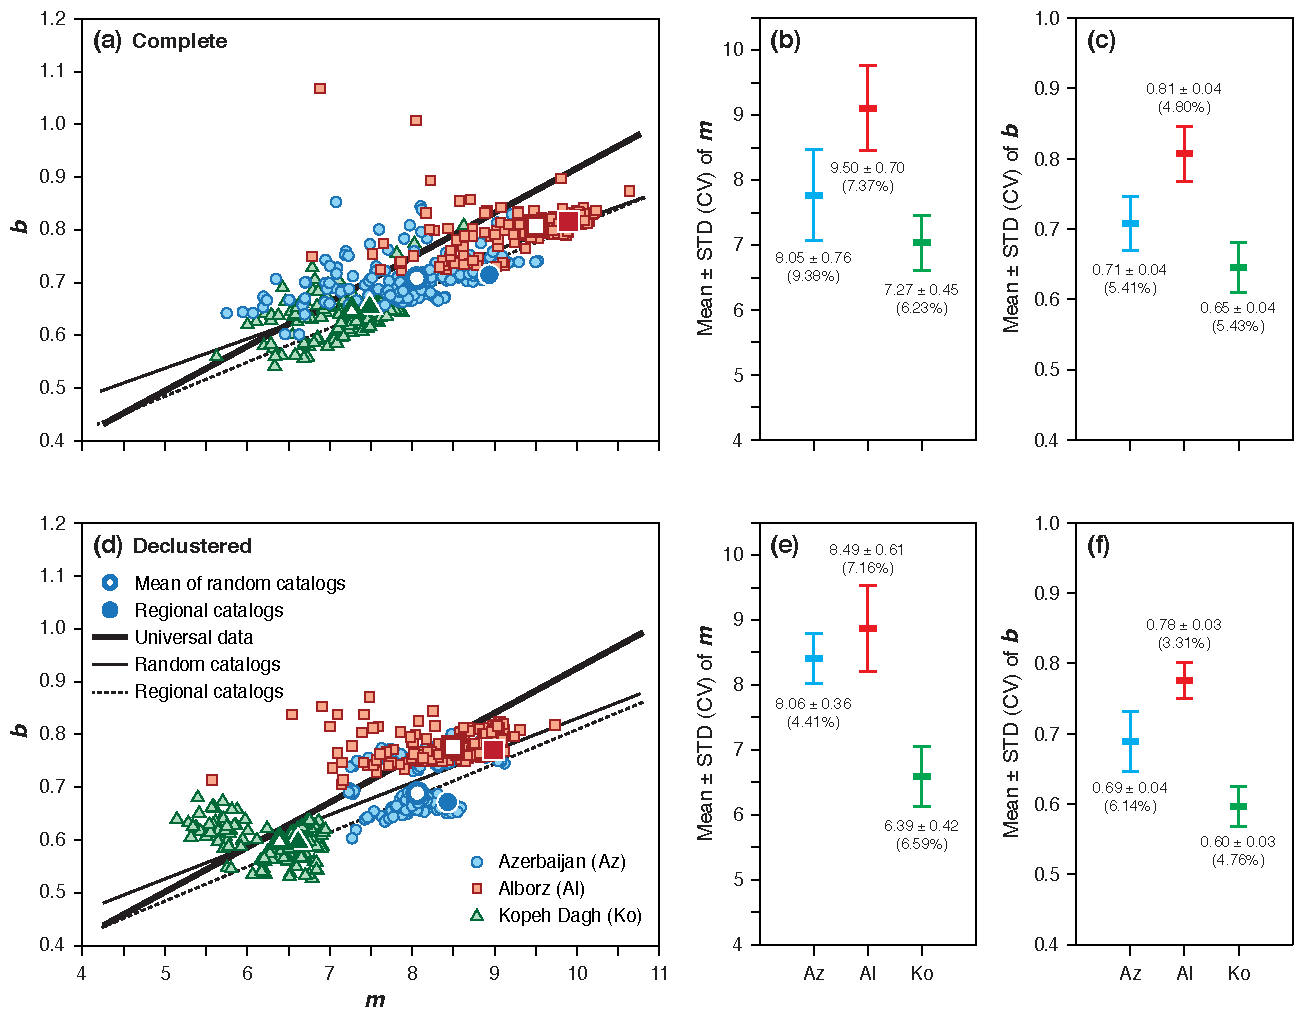
\includegraphics[width=\textwidth]{figures/pdf/figure-08} 
	\caption{\myrevision{Correlation between the $k$-$M$ slope ($m$) and $b$ values for 200 random sequences extracted from the complete (a) and declustered (d) catalogs of the three northern Iranian seismic regions considered in this study (scattered symbols), including the mean values (empty symbols with thick border) and the data points obtained from the regional analyses (solid symbols), along with the linear regressions of each sample as indicated in the legend; and mean $\pm1$ standard deviation bar plots for $m$ (b,e) and $b$ (c,f) for the complete and declustered catalogs, respectively. In the latter, the values in the parentheses corresponds to the coefficients of variation.}}
	\label{fig:random}
\end{figure*}

\myrevision{Fig.~\ref{fig:random} shows the results for this analysis on random subsequences for both the complete and declustered catalogs. In particular, Figs.~\ref{fig:random}a and \ref{fig:random}d show} scattered points for all the individual $m$ and $b$ pairs for all the subsequences that were randomly picked from the \myrevision{complete and declustered} catalogs of each region in northern Iran (small symbols)\myrevision{, respectively}. Figures \ref{fig:random}b \myrevision{and \ref{fig:random}e show the variability of $m$, and Figs.~\ref{fig:random}c and \ref{fig:random}f show the variability of $b$. These variability plots} show the mean values of each parameter for all the random subsequences and the amplitudes of $\pm 1$ standard deviation, as well as the coefficients of variation (in percentage). \myrevision{Figures \ref{fig:random}a and \ref{fig:random}d also include the data points corresponding to the regional analysis of the catalogs, the points corresponding to the mean values of $m$ and $b$, and the universal linear regression from equations (\ref{eq:universal.bm}) and (\ref{eq:universal.bm.dc}), as well as the linear regressions for northern Iran when using the full-sequence catalogs (dashed thin line) and the random subsequence catalogs (continuous thin line).}

\myrevision{In essence, the results in Fig.~\ref{fig:random} show that, despite the variability in the random subsequences and the differences in the computation of $M_c$, both of which are sources of additional uncertainty, the analysis produces an outcome in fair agreement with the universal relationships. Nonetheless, the analysis of the random subsequences in the complete catalogs produces some outliers, whereas the processing of the declustered subsequences tends to concentrate more evenly around the universal trend. Note that, likely due to the removal of foreshocks and aftershocks, the declustered random subsequences exhibit a clearer distinction between the three seismic zones.}

\myrevision{While these sequences do not represent the dominant seismicity pattern of the region, the comparison between the mean values of the random sequences analysis versus the complete catalogs (large, empty and solid symbols in Fig.~\ref{fig:random}) indicates that there exists only a small bias, which is well within the standard deviation of the different value samples. Note also that the values of $m$ in Fig.~\ref{fig:random} are slightly smaller when obtained with the random sequence analysis than when done for the regional sequences, whereas the $b$ values seem more stable. This explains why the regressions of the random subsequences are less steep than the universal regressions, in both cases. In a separate initial analysis, not included here for brevity, we observed that lower, less conservative selections of $M_c$ can lead to random subsequences that yield regressions in better agreement with the universal trend. Using lower values of $M_c$, however, may be misleading. In this sense, larger catalogs in better instrumented regions may shed light on the stability of the $m$-$b$ relationship, which is the reason we included the data point from \citet{Azizzadeh_2017_SSA} for southern California in Fig.~\ref{fig:regression}, which falls well in line with the universal regression.}

\begin{figure*}[t]
	\centering
	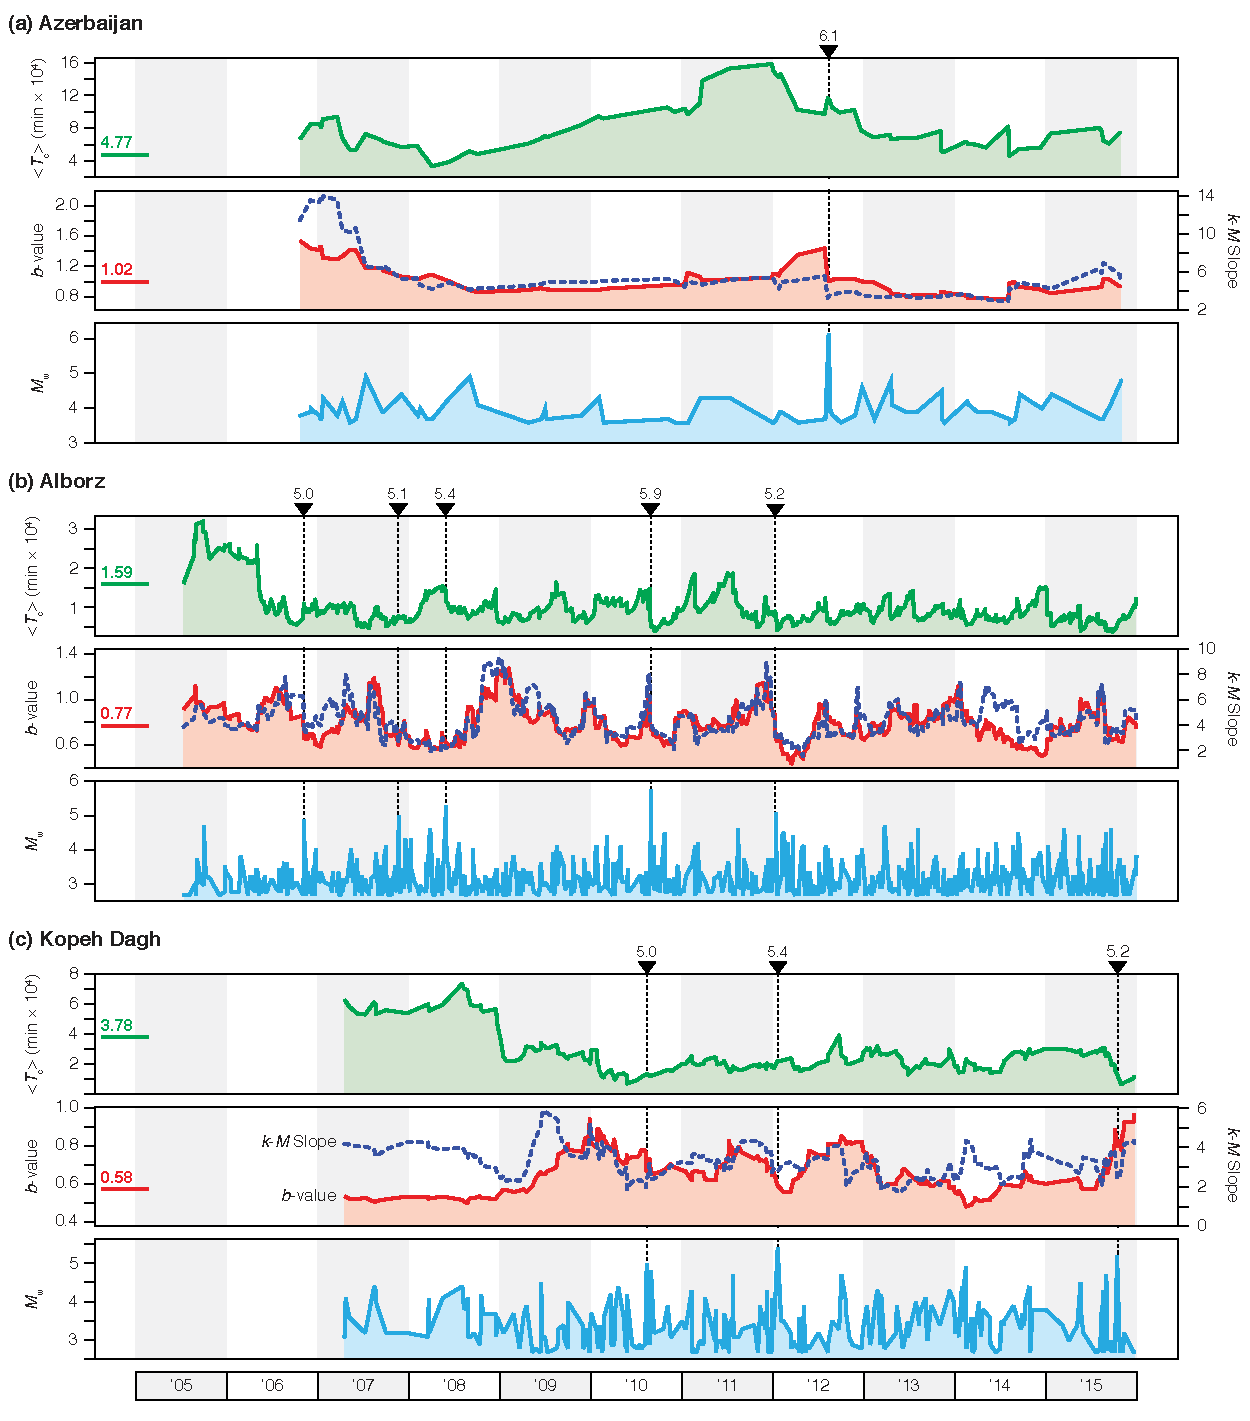
\includegraphics[width=\textwidth]{figures/pdf/figure-09} 
	\caption{\myrevision{Variation of $<$$T_c$$>$, $k$-$M$ slope ($m$) and the $b$ value with respect to time for the seismic zone of Alborz for a moving window analysis of the visibility graphs of subsequences of $n=50$ consecutive events, along with the magnitude and the connectivity degree ($k$) of events in the 2016 period. Black triangles indicate the occurrence of significant earthquakes in each of the regions, with the corresponding magnitude at the top of each symbol.}}
	\label{fig:tc}
\end{figure*}

We now investigate the relationship of the parameters obtained through the visibility graph analysis over time. Here, the visibility graph analysis is done by windows of equal number of events moving in time along the catalog sequence. The number of events in the window is kept fixed independently of the time between them, and the results are associated with the last event in the window. In this case, we are interested in using a small number of events to capture the relevance of each new event as the window moves in time. We tried different \myrevision{window sizes between 20 and 100 events per window for each seismic zone. As it is natural to expect, there are trade-offs between different window-sizes. Smaller window sizes emphasize the local changes in the time series, but are less reliable when it comes to the seismicity parameters (e.g., $b$ value). Larger window sizes, on the other hand, offer less insight into the time dependence of the window sequence characteristics. We chose a window size $n = 50$, which is consistent with the suggested minimum number of events acceptable to estimate $b$ according to \citet{Woessner_2005_BSSA}.}

\myrevision{In this windowing analysis, in addition to $b$ and $m$, we are interested in computing the value of $<$$T_c$$>$ explained in the Methodology section. Figure \ref{fig:tc} shows the earthquake sequence for the region of Alborz, and the variation of $k$, $m$, $b$, and $<$$T_c$$>$ with time. Although we performed the analysis for all three seismic zones, we concentrate in the region of Alborz because is the one with the larger number of events for the fixed-size moving window. We can see here how larger values of $k$ are associated with the larger magnitude earthquakes, and how the resulting values of $m$ for each 50-event sequence compares with $b$. In particular, we observe a good correlation between $m$ and $b$ fore the period prior to the 2010 $M_w$ 5.8 Damaghan earthquake, but after this event the correlation is not as clear. Unfortunately, contrary to the suggestions of \citet{Telesca2016}, we do not observe any clear correlation between the behavior of $<$$T_c$$>$ and the occurrence of the larger magnitude ($M_w \geq 5$) earthquakes in this region. Similarly, while the occurrence of larger events does seem to coincide with drops in $m$ and $b$, there are other similar changes in the values of $m$ and $b$ that are not associated with any significant event, making it difficult to draw strong conclusions. Nonetheless, in the region of Azerbaijan, we did observe more prominent changes in $m$ and $b$ with the occurrence of the 2012 $M_w$ 6.4 Tabriz earthquake, which leaves open the possibility of further study for regions with larger magnitude events.}

\begin{figure*}[t]
	\centering
	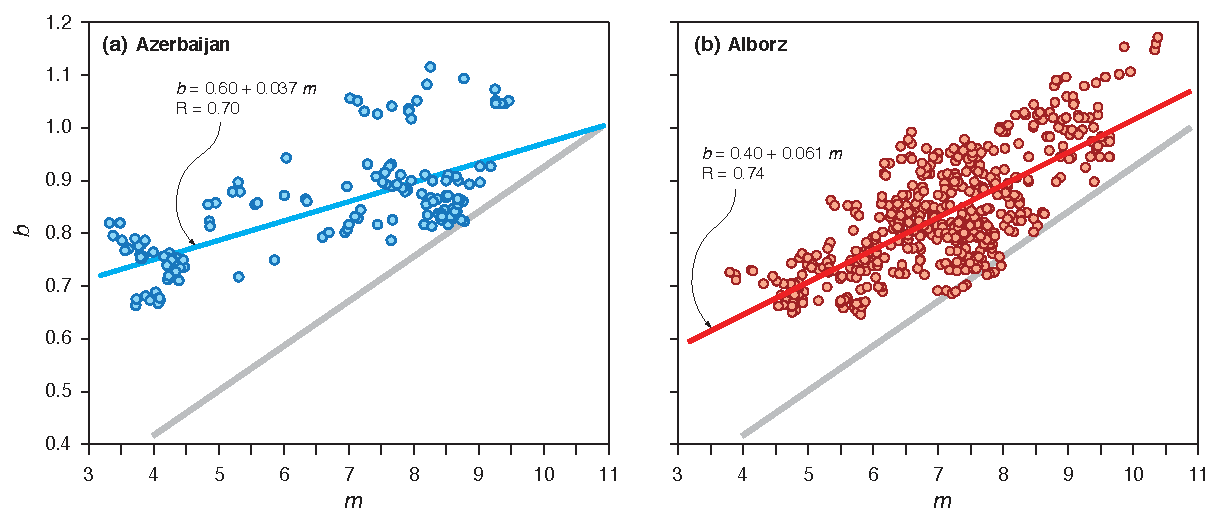
\includegraphics[width=\textwidth]{figures/pdf/figure-10} 
	\caption{\myrevision{Correlation between $m$ and $b$ based on the fixed-size windowing analysis done for the region of Alborz, for both the complete (a) and declustered (b) catalogs, along with the linear regressions of each case. While a direct comparison is not appropriate, the universal regression is shown as well for reference.}}
	\label{fig:alborz-bm}
\end{figure*}

\myrevision{Finally, we explore the correlation between $k$ and $b$ by aggregating the results of the windowing analysis. Figure \ref{fig:alborz-bm}a shows condensed (scattered) results for all the values $k$ and $b$ from Fig.~\ref{fig:tc} for the complete catalog of Alborz, and Fig.~\ref{fig:alborz-bm}b shows the same results but for the declustered catalog. Both plots exhibit reasonable linear regressions for an ample range of $m$ and $b$ values. While it is not entirely fair to compare these results (which are exclusive to the Alborz region) with the universal results discussed before, Fig.~\ref{fig:alborz-bm} also includes the universal correlations for reference. The results for Alborz also show $b$ to increase proportionally with $m$, although at a smaller rate.}

% OLD MATERIAL
% -----------------------------------------------------------------

% Another aspect of interest is the stability of the data points themselves. Note that as presented in Fig.~\ref{fig:regression}, the analysis of the sequences shown in Fig.~\ref{fig:mag-time} only contribute one data point per region of interest. Furthermore, each data-point comes from sequences that vary significantly in terms of the number of events and seismic parameters (see Table \ref{tab:seismicity}). 

% \myrevision{According to Scholtz (1968) b-value for microfractures in rocks is reported ranging between 0.11 and 2.58. Using different synthetic and real catalog, in this study we cover a broad range from low b-value (synthetics) to high b-value(subduction zone)}. 

% Fig.~\ref{fig:regression} also includes the results of different linear regressions between the $b$-value and the $k$-$M$ slope. Each regression reflects the addition of new data-points from different studies. Note that the regression improves as new data-points are added, which is indicated by the correlation coefficient $R$, also included in the figure. The correlation fitting various regional seismic data was previously pointed out by \citet{Telesca2014}.

% \cmmnt{Note also that the threshold value of $M_c$ is significantly smaller for Azerbaijan than for Alborz or Kopeh Dagh. This is due in part to the fact that the latter two zones were more seismically active in the time period under consideration} 
% \myrevision{In this study due to using windowing method, we consider a very conservative completeness magnitude}. However, according to \citet{Telesca2012}, the threshold magnitude has a minor effect in the graph parameters.

% Moving on, \citet{Telesca2013} observed that the value of the $k$-$M$ slope was not particularly sensitive to the sample size in the sequence---at least not when considering sufficiently large sequences. On the other hand, as we will see below, if the sequence window is sufficiently small, then the $k$-$M$ slope value shows a relative dependence on time and thus provides insight about the variation of the seismicity as the sequence progresses. 

% Note that the results of the whole catalog for each seismic region is different from Fig.~\ref{fig:regression}. In Fig.~\ref{fig:regression} we choose a time dependent completeness magnitude which is conservative and requires inspection. In order to keep uniformity in the random data test we computed the completeness magnitude through GFT for all subsamples and the whole catalog of each seismic region. Determination of completeness magnitude based on the best score of GFT between synthetic catalog and subsamples could be controversial. It is possible to choose very large $M_c$ just because of slightly higher GFT score than smaller magnitudes. This could result in a sequence of data where is not completely a representative of the domain. However, knowing these source of uncertainties, the randomly generated data conforms the fact that the method is fairly robust for the catalog size and completeness magnitude; where we can easily distinguish the 3 seismic region border. There are some outlier data due to subsamples of aftershocks of big earthquakes. These sequences represent different $k-M$ and $b-value$ relationship. These sequences do not represent the dominant seismicity pattern of the region. In the declustered catalog (is not presented here) we do not see these outliers.}

% \cmmnt{
% The comparisons of the regressions, however, indicate that the analysis of the random sub-catalogs leads to a result more in line with the universal results obtained when considering multiple seismic zones. The linear regression of the random sub-catalogs yields the following equation:
% % 
% \begin{equation}
%    	b = 0.045  +0.390 m \, .
% 	\label{eq:iran.bm}
% \end{equation}

% Note that equations (\ref{eq:universal.bm}) and (\ref{eq:iran.bm}) have similar intercepts with the $b$-value axis, and only slightly different slope constants. In this particular case, the analysis for northern Iran leads to a relationship in which the $b$-value increases more rapidly with $m$ than in the case of the regression obtained for the universal data. The similarity between the two equations, however, is a positive sign of the stability of the method.}

% each of the three seismic zones in northern Iran. The time-magnitude sequence is also included for reference. Note that the behavior of the $k$-$M$ slope and the $b$-value is very similar along time for all three zones. \myrevision{Specially in the case of Alborz where because of higher number of events the correlation is easily seen.} This is consistent with the results presented before. We note that there seems to be a correlation between the behavior of the $b$-value in time with the occurrence of some of these larger events. In particular, some of the events in the figure seem to coincide with a drop in the $b$-value. 

% The decline of the $b$-value before large earthquakes has been studied in other regions before \citep[e.g.,][]{Wyss2000, Wyss2006, Schorlemmer2005, Chan2012}. In the context of the visibility graph analysis, \citet{Telesca2016} observed a decrease in <$T_c$> before the large earthquake of the western India earthquake sequence. We recognize, however, that the lack of larger ($M>6$) events in our region of interest in the last decade prevents us from drawing a stronger conclusion on this regard. 

